\documentclass{beamer}

\usepackage[utf8]{inputenc}
\usecolortheme{beaver}
\usepackage{caption}
\usepackage{subcaption}
\usepackage{mathtools}
\usepackage{todonotes}
\usepackage{bm}

\def\ci{\perp\!\!\!\!\!\perp}

\newtheorem{proposition}{Proposition}

\begin{document}

\title{A Simple Unified Approach to Testing High-Dimensional Conditional
Independencies for Categorical and Ordinal Data}
\author {Ankur Ankan \and Johannes Textor}
\date{}
\maketitle

\begin{frame}
	\frametitle{Overview}
	\tableofcontents
\end{frame}

\section{Motivation}
\begin{frame}
	\frametitle{Motivation: Example DAG / Causal Bayesian Network}
	\begin{figure}
		\centering
		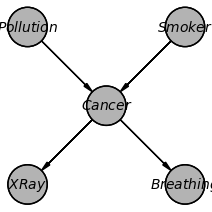
\includegraphics[scale=0.6]{imgs/example_dag.png}
		\caption*{An example Directed Acyclic Graph (DAG)}
	\end{figure}
	\begin{itemize}
		\setlength\itemsep{1em}
		\item Random variables are represented using nodes.
		\item Directed edges represent direct causal link between variables.
		\item DAGs imply Conditional Independencies (CI). Eg:
			\hspace*{20pt} $ \text{\emph{Pollution}} \ci \text{\emph{XRay}} | \text{\emph{Cancer}} $ \newline
			\hspace*{20pt} $ \text{\emph{XRay}} \ci \text{\emph{Breathing}} | \text{\emph{Cancer}} $
	\end{itemize}
\end{frame}

\begin{frame}
	\frametitle{Motivation: Model Testing}
	\begin{itemize}
		\setlength\itemsep{1em}
		\item In applied research, most of the DAGs are made by hand
			based on domain knowledge.
		\item Important to test whether model is consistent with the data.
		\item Implied CIs can be tested in the dataset to verify
			model structure.
		\item Unlike scoring based methods, CI testing can give
			information on exactly what part of the model isn't
			consistent.
	\end{itemize}

\end{frame}

\begin{frame}
	\frametitle{Motivation: Structure Learning}
	\begin{itemize}
		\setlength\itemsep{1em}
		\item CI implies that no direct causal link exists between the variables. \newline
		\hspace*{20pt} $ \text{\emph{Pollution}} \ci \text{\emph{XRay}} | \text{\emph{Cancer}} \implies \text{\emph{Pollution}} \not \rightarrow  \text{\emph{XRay}} $

		\todo[inline]{This shouldn't be directed edge. Make it undirected}

		\item Constraint-Based structure learning algorithms like PC
			and FCI systematically search for these independencies
			in the dataset to determine model skeletons.
	\end{itemize}
\end{frame}

\section{Background}
\begin{frame}
	\frametitle{(Conditional) Independence Test}
	\begin{block}{Independence Test}
		Two random variables $ X $ and $ Y $ are independent,
		$ X \ci Y $ if and only if $ P(X, Y) = P(X) \cdot P(Y) $.
	\end{block}
	\vspace{1em}

	\begin{block}{Conditional Independence Test} Two random variables $ X $
		and $ Y $ and are said to be conditionally independent given $
		\bm{Z} $, $ X \ci Y | \bm{Z} $ if and only if for all $ z $
		with $ p(z) > 0 $, $ P(X, Y | Z=z) = P(X | Z=z) \cdot P(Y |
		Z=z) $
	\end{block}
\end{frame}

\begin{frame}
	\frametitle{CI Testing is Difficult}
	\begin{itemize}
		\setlength\itemsep{1em}
		\item Normal non-conditional independence testing is easy.
			Things like exact tests are available. \todo[inline]{Need to make the argument stronger here}
		\item Conditional indpendence testing is a hard.
		\item For continous conditional variables, has been proven that no single 
		      test exists which has power against all datasets. \footnotemark
		\item But also well studied problem, and many approaches/tests exist.
	\end{itemize}

	\footnotetext[1]{\footnotesize{Shah, Rajen D., and Jonas Peters. "The hardness of conditional independence testing and the generalised covariance measure." The Annals of Statistics 48.3 (2020): 1514-1538.}}
\end{frame}

\begin{frame}
	\frametitle{Main classes of tests}
	\begin{itemize}
		\setlength\itemsep{1em}
		\item Stratification based tests
		\item Variable Importance based tests
		\item Residulaization based tests
	\end{itemize}
\end{frame}

\begin{frame}
	\frametitle{Stratification Based Tests}
	\begin{itemize}
		\setlength\itemsep{1em}
		\item Most common type for discrete variables. Eg. chi-squared,
			mutual information etc. 
		\item Converts CI test into simple independence test by splitting 
			the dataset.
		$ D[X, Y, \bm{Z}] = \{ D[X, Y, \bm{Z}=\bm{z_1}, D[X, Y, \bm{Z}=\bm{z_2}], \cdots \} $	
		\item Runs test on each of the stratum and then combines the results.
		\item Exponenially less data is available in each stratum as 
			number of conditional variables increase.
		\item Looses power when number of conditonal variables
			are increased.
	\end{itemize}
\end{frame}

\begin{frame}
	\frametitle{Variable Importance Tests}
	\begin{itemize}
		\setlength\itemsep{1em}
		\item Based on comparing the probability models: $\hat{p}(x | y, z) $ 
			and $ \hat{p}(x | z) $.
		\item $ \hat{p}(x|y, z) $ and $ \hat{p}(x | z) $ is estimated using a
			statistical model, and if the simpler model doesn't fit
			significantly worse, $ X \ci Y | Z $ is True.
		\item An example is SCCI, which is the current state-of-the-art
			for structure learning in discrete variables.
		\item Can utilize any statistical model for which a reasonable goodness
			of fit exist.
		\item Inherently asymmetrical. The result of $ X \ci Y | Z $
			can be different from $ Y \ci X | Z $.
	\end{itemize}

\end{frame}

\begin{frame}
	\frametitle{Residualization Based Tests}
	\todo[inline]{Improve this slide}
	\begin{itemize}
		\setlength\itemsep{1em}
		\item Example: partial correlation test.
		\item Fits two models $ \mathbb{E}[X | Z] $ and $ \mathbb{E}[Y | Z] $.
		\item Compute residuals $ R_{X|Z} $ and $ R_{Y|Z} $.
		\item Under CI, if $ \mathbb{E}[R_{X|Z}] = \mathbb{E}[R_{Y|Z}] = 0 $, the
			$ \mathbb{E}[R_{X|Z}R_{Y|Z}] = 0 $. \footnotemark
	\end{itemize}
	\footnotetext[1]{\footnotesize Daudin, J. J. "Partial association measures and an application to qualitative regression." Biometrika 67.3 (1980): 581-590.}
\end{frame}

\section{Proposed Method}
\begin{frame}
	\frametitle{Proposed Method: Random Forest Based Test (RFT)}
	\begin{itemize}
		\setlength\itemsep{1em}
		\item Residualization based approach.
		\item Any unbaised estimator can be used.
		\item Uses Lee-Shepherd residuals.
		\item Gives a chi-square distributed test statistic.
	\end{itemize}
\end{frame}

\begin{frame}
	\frametitle{Lee-Shepherd (LS) Residuals}
	\todo[inline]{Add paper in the footnote. Also the notation isn't correct.}
	Given a sample $ \bm{y} $ of $ Y $ and an estimate $ \hat{p}(y) $ of $ p(y) $,
	LS-Residual is defined as:
	$$ R_{y_i} = \hat{p}(Y < y_i) - \hat{p}(Y > y_i) $$
	\vspace{1em}

	For the binary case with $ Y \in \{0, 1\} $:
	$$ R_{y_i} = y_i - \hat{p}(Y = 1) $$
	\vspace{1em}

	For the conditional case for sample $ (\bm{y}|\bm{z})_i $,
	$$ R_{y_i | z_i} = \hat{p}(Y < y_i | Z=z_i) - \hat{p}(Y>y_i|Z=z_i) $$

	Property: For unbaised estimators, LS-Residuals satisfy: $ E[R_{x|z}] =
		E[R_{y|z}] = 0 $.
\end{frame}

\begin{frame}
	\frametitle{Proposition 1}
	If $ X \ci Y | Z $ and $ \hat{p}(x|z) $ and $ \hat{p}(y|z) $ are asymptotically
	unbiased estimators of $ p(x|z) $ and $ p(y|z) $ respectively, then 
	$ \mathrm{Cov}(R_{x|z}, R_{y|z}) = 0 $.	
	\vspace{1em}

	\begin{itemize}
		\setlength\itemsep{1em}
		\item For unbaised estimators, LS-Residuals satisfy:
			$ E[R_{x|z}] = E[R_{y|z}] = 0 $.
		\item From Daudin(1980), if $ X \ci Y | \bm{Z} $ with residual exectations
			as $ 0 $, $ \mathbb{E}[R_{x|z} R_{y|z}] = 0 $.
	\end{itemize}
\end{frame}

\begin{frame}
	\frametitle{Test Statistic: Both ordinal variables}
	$$ Q_1(\bm{x}, \bm{y}) = \frac{1}{n} \frac{(R_{\bm{x}} \cdot R_{\bm{y}})^2}{\bm{var}(R_{\bm{x}} R_{\bm{y}})} $$

	If $ X \ci Y | Z $, then asymptotically $ Q_1(\bm{x}, \bm{y}) \sim \chi^2(1) $.

	\begin{itemize}
		\setlength\itemsep{1em}
		\item Square of sample mean of $ R_x R_y $ divided by its
			standard deviation.
		\item From Proposition 1, the population mean is 0 under CI.
		\item Using CLT, the standardized sample mean is asymptotically
			standard normal.
		\item Square of standard normal distribution gives a
			chi-squared distribution with $ 1 $ degree of freedom.
	\end{itemize}
\end{frame}

\begin{frame}
	\frametitle{Test Statistic: One ordinal and one categorical}
	$$ Q_2(\bm{x}, \bm{y}) = \frac{1}{n} (d \times \hat{\Sigma}_d^{-1} \times d^T) $$

	where $ d = (R_{\mathbb{I}(\mathbf{x}=1)} \cdot R_{\mathbf{y}}, \, \ldots \ ,
		R_{\mathbb{I}(\mathbf{x}=k-1)} \cdot R_{\mathbf{y}})$.
	If $ X \ci Y | Z $, then asymptotically $ Q_1(\bm{x}, \bm{y}) \sim \chi^2(k-1) $.
	\begin{itemize}
		\setlength\itemsep{1em}
		\item Dummy/One-hot encode the categorical variable.
		\item Under CI, each component of $ d $ is asymptotically normal.
		\item Hence, $ d $ is multivariate gaussian.
		\item $ \sqrt{(Q_2(\bm{x}, \bm{y}))} $ is multivariate standard normal.
		\item $ Q_2 $ is chi-square distributed with $ k-1 $ dof.
	\end{itemize}
\end{frame}

\begin{frame}
	\frametitle{Test Statistic: Both categorical}
	Both categorical variables with $ k $ and $ r $ categories.


	$$ Q_3(\bm{x}, \bm{y}) = \frac{1}{n} (d \times \hat{\Sigma}_d^{-1} \times d^T) $$

	If $ X \ci Y | Z $, then asymptotically $ Q_1(\bm{x}, \bm{y}) \sim
	\chi^2((k-1)(r-1)) $.

	\todo[inline]{Fix the value of $ d $}
	where $ d = (R_{\mathbb{I}(\mathbf{x}=1)} \cdot R_{\mathbf{y}}, \, \ldots \ ,
		R_{\mathbb{I}(\mathbf{x}=k-1)} \cdot R_{\mathbf{y}}) $.

	\begin{itemize}
		\setlength\itemsep{1em}
		\item Same as the last case, $ Q_3(\bm{x}, \bm{y}) $ is chi square distributed 
			with $ (k-1)(r-1) $ dof.
	\end{itemize}
\end{frame}

\begin{frame}
	\frametitle{Test Summary / Algorithm}
	\begin{enumerate}
		\setlength\itemsep{1em}
		\item If either $ X $ or $ Y $ are non-binary categorical,
			dummy/one-hot encode them.
		\item Train two random forest classifiers $ C_x = X \sim \bm{Z} $ and
			$ C_y = Y \sim \bm{Z} $
		\item Make probability predictions using these two classifiers
			$ \hat{p}(X) = C_x(\bm{Z}) $ and $ \hat{p}(Y) =
			C_y(\bm{Z}) $.
		\item Use predictions and true values to compute LS-Residuals $ R_{x|z} $ and $ R_{y|z} $.	
		\item Compute covariance matrix on the product of the residuals
		\item Compute the test statistic and degrees of freedom(dof).
	\end{enumerate}
\end{frame}

\begin{frame}
	\frametitle{Properties of RFT}
	\begin{itemize}
		\setlength\itemsep{1em}
		\item Simple to implement
		\item Interpretable chi-square test statistic
		\item Symmetric by construction
		\item Computationally feasible
	\end{itemize}
\end{frame}

\section{Empirical Results}

\begin{frame}
	\frametitle{Empirical Analysis: Calibration}
	\begin{figure}
		\centering
		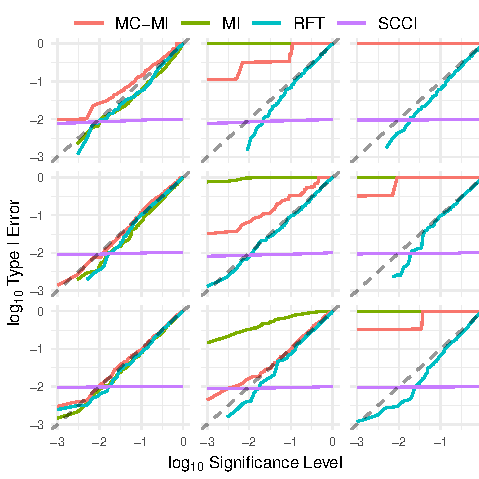
\includegraphics[scale=0.8]{imgs/calibration_add_vars.pdf}
		\caption*{Type I error vs significance level for sample sizes (top to
		bottom): $ [20, 40, 80] $ and number of conditional variables (left to
		right): $ [1, 3, 5] $ on conditionally independent simulated binary
		datasets.}
	\end{figure}
\end{frame}

\begin{frame}
	\frametitle{Empirical Analysis: Discrimination}
	\begin{figure}
		\centering
		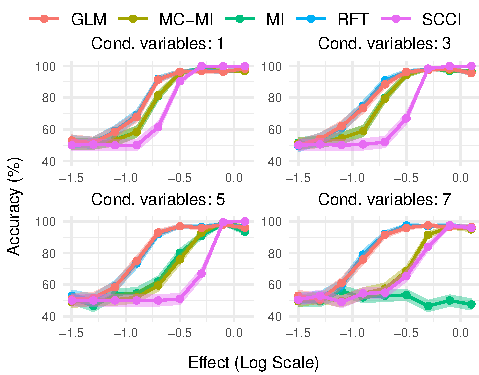
\includegraphics{imgs/accuracy.pdf}
		\caption*{Accuracy (shading: mean $\pm$ standard error, $N=200$)
		of classifying simulated binary datasets (sample size: $1000$)
		as conditionally dependent or independent.}
	\end{figure}
\end{frame}

\begin{frame}
	\frametitle{Empirical Analysis: Discrimination}
	\begin{figure}
		\centering
		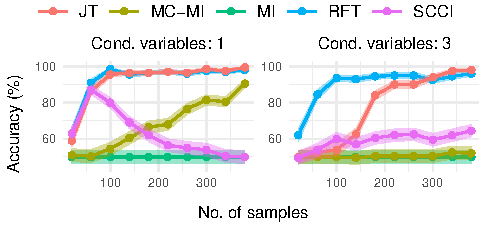
\includegraphics{imgs/accuracy_ordinal.pdf}
		\caption*{Accuracy (shading: mean $\pm$ standard error) of
		classifying simulated ordinal data (8 levels per variable) as
		conditionally dependent or independent.}	
	\end{figure}
	\todo[inline]{Mention what test JT is here}
\end{frame}

\begin{frame}
	\frametitle{Applications: Model testing}
	\begin{figure}
		\centering
		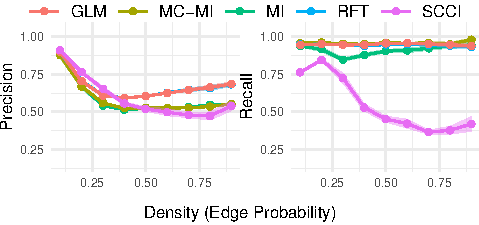
\includegraphics{imgs/model_testing.pdf}
		\caption*{Precision and recall (shading: mean $\pm$ standard
		error) of testing implied CIs and equal number of randomly
		generated CIs in binary datasets (sample size: $1000$)
		simulated from random DAGs on $ 20 $ variables.}
	\end{figure}
\end{frame}

\begin{frame}
	\frametitle{Applications: Structure Learning}
	\begin{figure}
		\centering
		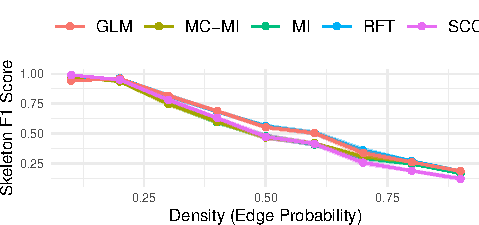
\includegraphics{imgs/sl_density.pdf}
		\caption*{Structure learning on simulated data. F1-score
		(shading: mean $\pm$ standard error) of the learned model
		skeletons for randomly generated DAGs with $20$ variables and
		varying edge probabilities.  Binary datasets of $ 1000 $
		samples are simulated from the DAGs using logistic models with
		all coefficients set to $ 0.15$.}
	\end{figure}
\end{frame}

\begin{frame}
	\frametitle{Applications: Structure Learning}
	\begin{figure}
		\centering
		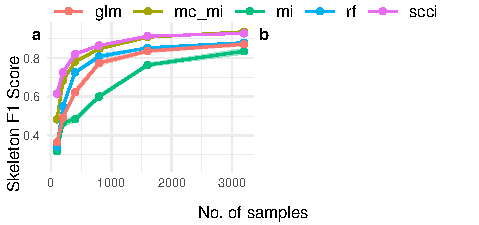
\includegraphics{imgs/sl.pdf}
		\caption*{Structure learning on (a) ``alarm'', and (b)
		``insurance'' datasets.  F1-score (shading: mean $\pm$ standard
		error, $N=10$) of the learned model skeletons.  Presence of an
		edge is considered the "positive" case for computing the
		F1-Scores.}
	\end{figure}
\end{frame}

\begin{frame}
	\frametitle{Applications: Structure Learning}
	\begin{figure}
		\centering
		\begin{subfigure}{0.5\textwidth}
			\centering
			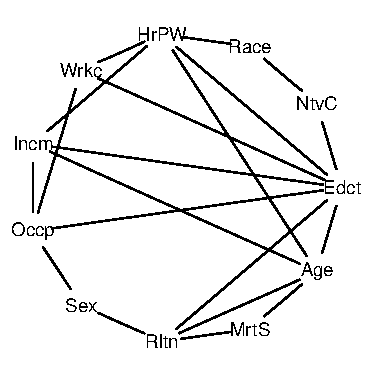
\includegraphics[scale=0.85]{imgs/sl-adult-rf.pdf}
			\caption*{}
			\label{fig:sl_adult_model}
		\end{subfigure}%
		\begin{subfigure}{0.5\textwidth}
			\centering
			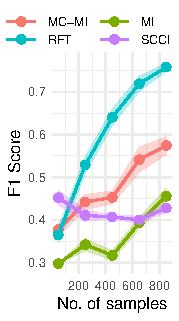
\includegraphics{imgs/adult_F1.pdf}
			\caption*{}
			\label{fig:sl_adult}
		\end{subfigure}
		\caption*{Structure learning on US census income dataset. (a)
		Learnt skeleton using RFT. (b) F1-score (shading: mean $\pm$
		standard error, $N=10$) when comparing $d$-connected variable
		pairs from the CPDAG to correlated variable pairs in the
		dataset.}
	\end{figure}
\end{frame}

\begin{frame}
	\frametitle{Runtime Analysis}
	\begin{figure}
		\centering
		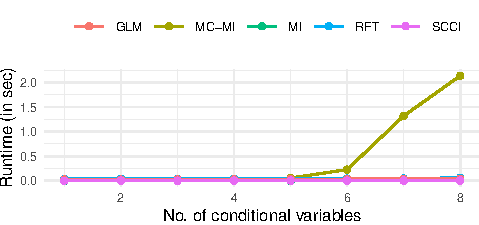
\includegraphics{imgs/runtime.pdf}
		\caption*{Runtime (shading: mean $\pm$ standard error, $N=100$)
		for CI tests with varying numbers of conditional variables and
		$1000$ samples per dataset.
		}
	\end{figure}
\end{frame}

\section{Conclusion}
\begin{frame}
	\frametitle{Conclusion/Future Work}
	\begin{itemize}
		\setlength\itemsep{1em}
		\item A simple test which performs reasonably well for low number of
			conditional variable but performs better for high number of
			conditional variables.
		\item For structure learning, a hybrid approach can be used with other
			tests.
		\item Since Random Forest can work with combination of discrete and 
			continuous variables, can possibly be extended to a single 
			unified test.
	\end{itemize}
\end{frame}

\begin{frame}
	Questions / Suggestions
\end{frame}

\end{document}
